\documentclass[11pt,a4paper]{article}

\usepackage[utf8]{inputenc}
\usepackage[margin=1in]{geometry}
\usepackage{graphicx}
\usepackage{hyperref}
\usepackage{xcolor}
\usepackage{listings}
\usepackage{booktabs}
\usepackage{tikz}
\usepackage{amsmath}
\usepackage{amssymb}
\usepackage{pgfplots}
\pgfplotsset{compat=1.17}
\usetikzlibrary{shapes.geometric, arrows, positioning, fit, calc, decorations.pathreplacing, backgrounds, shadows}

% Colors matching presentation theme
\definecolor{primaryblue}{RGB}{46, 134, 171}
\definecolor{darkbg}{RGB}{55, 65, 81}
\definecolor{lightbg}{RGB}{75, 85, 99}
\definecolor{accentgold}{RGB}{212, 175, 55}
\definecolor{successgreen}{RGB}{34, 197, 94}
\definecolor{warningred}{RGB}{214, 40, 40}
\definecolor{warningorange}{RGB}{247, 127, 0}
\definecolor{codebg}{RGB}{245, 245, 245}
\definecolor{isoforest}{RGB}{99, 102, 241}
\definecolor{xgboost}{RGB}{16, 185, 129}
\definecolor{histgrad}{RGB}{245, 158, 11}
\definecolor{ocsvm}{RGB}{239, 68, 68}

% Hyperlink styling
\hypersetup{
    colorlinks=true,
    linkcolor=primaryblue,
    urlcolor=primaryblue
}

% Code listing style
\lstset{
    backgroundcolor=\color{codebg},
    basicstyle=\ttfamily\small,
    breaklines=true,
    frame=single,
    rulecolor=\color{gray},
    language=Python,
    keywordstyle=\color{primaryblue}\bfseries,
    commentstyle=\color{gray},
    stringstyle=\color{successgreen}
}

\title{\textbf{Anomaly Detection \& Agentic AI}\\[0.5em]\large Technical Documentation \& Presentation Materials\\[0.3em]\normalsize Receipt Automation Pipeline - Think Agentically}
\author{Luke Hartfield, John MacDonald, Emily Caraher,\\Raghu Subramanian, Michael Ovassapian}
\date{December 2025}

\begin{document}

\maketitle

\begin{center}
\fbox{\parbox{0.9\textwidth}{
\textbf{Overleaf Note:} This document expects images in an \texttt{images/} folder at the project root. \\
Required images: \texttt{anomaly\_detection\_evaluation.png}, \texttt{anomaly\_model\_comparison.png}, \texttt{anomaly\_confusion\_matrix.png}, \texttt{pipeline\_summary.png}
}}
\end{center}

\tableofcontents
\newpage

% ============================================================================
\section{Anomaly Detection}
% ============================================================================

The Anomaly Detection module is responsible for identifying suspicious or fraudulent receipts before they are auto-approved. This section covers our ensemble approach combining multiple detection strategies.

\subsection{Problem Statement}

Receipt fraud and errors manifest in various ways:
\begin{itemize}
    \item \textbf{Unusually high amounts} (e.g., \$50,000 for a coffee shop)
    \item \textbf{Missing critical fields} (no vendor name, invalid dates)
    \item \textbf{Suspicious patterns} (transactions at unusual hours, repeated round numbers)
    \item \textbf{Data integrity issues} (negative totals, impossible dates like 99/99/9999)
\end{itemize}

\subsection{Ensemble Architecture}

We combine four distinct anomaly detection approaches, each with different strengths:

% ============================================================================
% SLIDE IMAGE 1: Ensemble Voting Mechanism
% ============================================================================
\begin{figure}[h]
\centering
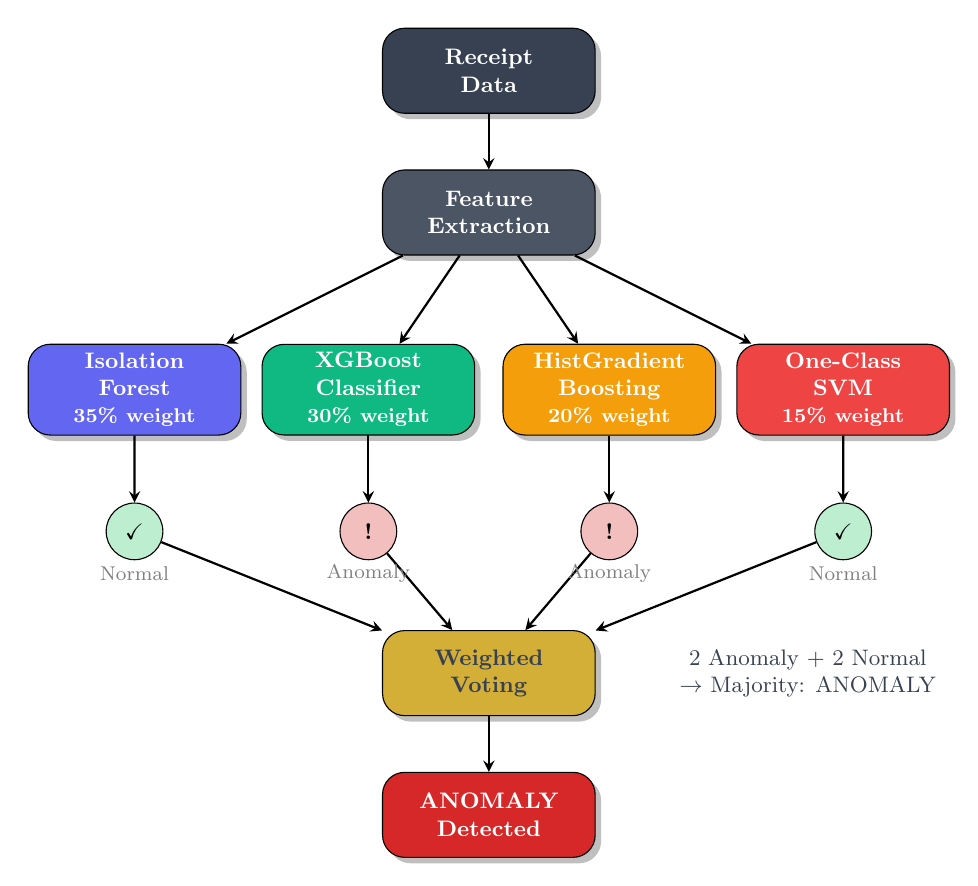
\begin{tikzpicture}[
    scale=0.9,
    transform shape,
    model/.style={rectangle, draw, rounded corners=8pt, minimum width=3cm, minimum height=1.2cm, align=center, font=\small\bfseries, drop shadow},
    vote/.style={circle, draw, minimum size=0.8cm, font=\small\bfseries},
    arrow/.style={->, thick, >=stealth},
    darrow/.style={->, thick, >=stealth, dashed}
]
    % Input Receipt
    \node[model, fill=darkbg, text=white] (input) at (0, 0) {Receipt\\Data};
    
    % Feature Extraction
    \node[model, fill=lightbg, text=white] (features) at (0, -2) {Feature\\Extraction};
    
    % Four Models
    \node[model, fill=isoforest, text=white] (iso) at (-5, -4.5) {Isolation\\Forest\\{\footnotesize 35\% weight}};
    \node[model, fill=xgboost, text=white] (xgb) at (-1.7, -4.5) {XGBoost\\Classifier\\{\footnotesize 30\% weight}};
    \node[model, fill=histgrad, text=white] (hist) at (1.7, -4.5) {HistGradient\\Boosting\\{\footnotesize 20\% weight}};
    \node[model, fill=ocsvm, text=white] (svm) at (5, -4.5) {One-Class\\SVM\\{\footnotesize 15\% weight}};
    
    % Voting circles
    \node[vote, fill=successgreen!30] (v1) at (-5, -6.5) {\checkmark};
    \node[vote, fill=warningred!30] (v2) at (-1.7, -6.5) {!};
    \node[vote, fill=warningred!30] (v3) at (1.7, -6.5) {!};
    \node[vote, fill=successgreen!30] (v4) at (5, -6.5) {\checkmark};
    
    % Weighted Voting
    \node[model, fill=accentgold, text=darkbg] (voting) at (0, -8.5) {Weighted\\Voting};
    
    % Final Decision
    \node[model, fill=warningred, text=white] (decision) at (0, -10.5) {ANOMALY\\Detected};
    
    % Arrows from input to features
    \draw[arrow] (input) -- (features);
    
    % Arrows from features to models
    \draw[arrow] (features) -- (iso);
    \draw[arrow] (features) -- (xgb);
    \draw[arrow] (features) -- (hist);
    \draw[arrow] (features) -- (svm);
    
    % Arrows from models to votes
    \draw[arrow] (iso) -- (v1);
    \draw[arrow] (xgb) -- (v2);
    \draw[arrow] (hist) -- (v3);
    \draw[arrow] (svm) -- (v4);
    
    % Arrows from votes to voting
    \draw[arrow] (v1) -- (voting);
    \draw[arrow] (v2) -- (voting);
    \draw[arrow] (v3) -- (voting);
    \draw[arrow] (v4) -- (voting);
    
    % Arrow to decision
    \draw[arrow] (voting) -- (decision);
    
    % Labels
    \node[font=\footnotesize, text=gray] at (-5, -7.1) {Normal};
    \node[font=\footnotesize, text=gray] at (-1.7, -7.1) {Anomaly};
    \node[font=\footnotesize, text=gray] at (1.7, -7.1) {Anomaly};
    \node[font=\footnotesize, text=gray] at (5, -7.1) {Normal};
    
    % Voting explanation
    \node[font=\small, text=darkbg, align=center] at (4.5, -8.5) {2 Anomaly + 2 Normal\\$\rightarrow$ Majority: ANOMALY};
    
\end{tikzpicture}
\caption{Ensemble Anomaly Detection with Weighted Voting Mechanism}
\label{fig:ensemble-voting}
\end{figure}

\newpage

% ============================================================================
% SLIDE IMAGE 2: Feature Extraction Pipeline
% ============================================================================
\begin{figure}[h]
\centering
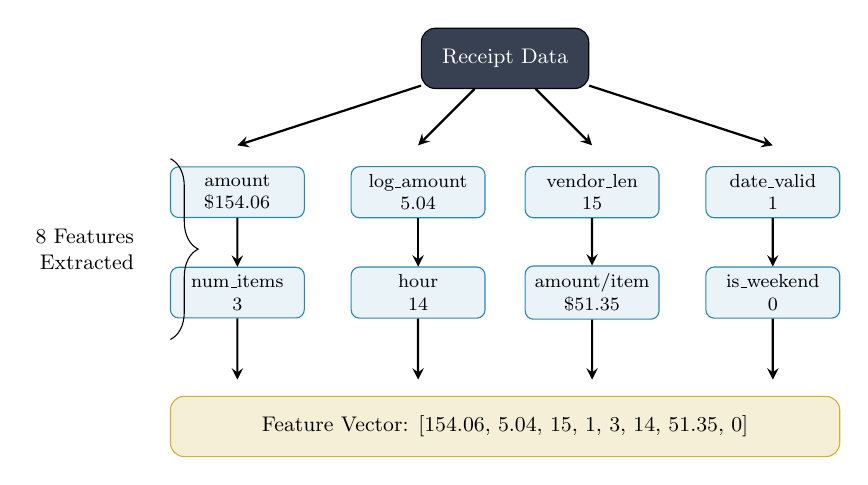
\begin{tikzpicture}[
    scale=0.85,
    transform shape,
    box/.style={rectangle, draw, rounded corners=5pt, minimum width=2.5cm, minimum height=0.9cm, align=center, font=\small},
    feature/.style={rectangle, draw=primaryblue, fill=primaryblue!10, rounded corners=3pt, minimum width=2cm, minimum height=0.7cm, align=center, font=\footnotesize},
    arrow/.style={->, thick, >=stealth}
]
    % Receipt input
    \node[box, fill=darkbg, text=white] (receipt) at (0, 0) {Receipt Data};
    
    % Feature boxes arranged in a grid
    \node[feature] (f1) at (-4, -2) {amount\\\$154.06};
    \node[feature] (f2) at (-1.3, -2) {log\_amount\\5.04};
    \node[feature] (f3) at (1.3, -2) {vendor\_len\\15};
    \node[feature] (f4) at (4, -2) {date\_valid\\1};
    
    \node[feature] (f5) at (-4, -3.5) {num\_items\\3};
    \node[feature] (f6) at (-1.3, -3.5) {hour\\14};
    \node[feature] (f7) at (1.3, -3.5) {amount/item\\\$51.35};
    \node[feature] (f8) at (4, -3.5) {is\_weekend\\0};
    
    % Feature vector
    \node[box, fill=accentgold!20, draw=accentgold, minimum width=10cm] (vector) at (0, -5.5) {Feature Vector: [154.06, 5.04, 15, 1, 3, 14, 51.35, 0]};
    
    % Arrows
    \draw[arrow] (receipt) -- (-4, -1.3);
    \draw[arrow] (receipt) -- (-1.3, -1.3);
    \draw[arrow] (receipt) -- (1.3, -1.3);
    \draw[arrow] (receipt) -- (4, -1.3);
    
    \draw[arrow] (f1) -- (f5);
    \draw[arrow] (f2) -- (f6);
    \draw[arrow] (f3) -- (f7);
    \draw[arrow] (f4) -- (f8);
    
    \draw[arrow] (f5) -- (-4, -4.8);
    \draw[arrow] (f6) -- (-1.3, -4.8);
    \draw[arrow] (f7) -- (1.3, -4.8);
    \draw[arrow] (f8) -- (4, -4.8);
    
    % Brace
    \draw[decorate, decoration={brace, amplitude=10pt, mirror}] (-5, -4.2) -- (-5, -1.5) node[midway, left=12pt, font=\small, align=right] {8 Features\\Extracted};
    
\end{tikzpicture}
\caption{Feature Extraction from Receipt Data}
\label{fig:feature-extraction}
\end{figure}

\subsection{Model Components}

\begin{table}[h]
\centering
\begin{tabular}{llcc}
\toprule
\textbf{Model} & \textbf{Type} & \textbf{Weight} & \textbf{Strength} \\
\midrule
Isolation Forest & Unsupervised & 35\% & Statistical outliers \\
XGBoost & Supervised & 30\% & Learned fraud patterns \\
HistGradientBoosting & Supervised & 20\% & NaN-robust, fast \\
One-Class SVM & Semi-supervised & 15\% & Decision boundary \\
\bottomrule
\end{tabular}
\caption{Ensemble Model Components and Weights}
\end{table}

\subsubsection{Why These Four Models?}

\begin{itemize}
    \item \textbf{Isolation Forest}: Works without labeled data. Detects receipts that are ``easy to isolate'' from normal patterns.
    \item \textbf{XGBoost}: Learns from known fraud examples. Catches patterns humans have identified before.
    \item \textbf{HistGradientBoosting}: Handles missing data natively. Robust when OCR fails to extract some fields.
    \item \textbf{One-Class SVM}: Creates a boundary around ``normal'' receipts. Anything outside is suspicious.
\end{itemize}

\subsection{Voting Formula}

The ensemble score is calculated as:

\begin{equation}
\text{score}_{\text{ensemble}} = \frac{\sum_{i=1}^{4} w_i \cdot s_i}{\sum_{i=1}^{4} w_i}
\end{equation}

where $w_i$ is the model weight and $s_i$ is the individual anomaly score.

Final classification uses majority voting:
\begin{equation}
\text{is\_anomaly} = \begin{cases}
\text{True} & \text{if } \sum_{i=1}^{4} \mathbf{1}[\text{model}_i = \text{anomaly}] \geq 2 \\
\text{False} & \text{otherwise}
\end{cases}
\end{equation}

\newpage

% ============================================================================
% SLIDE IMAGE 3: Anomaly Detection Reasons (Explainability)
% ============================================================================
\begin{figure}[h]
\centering
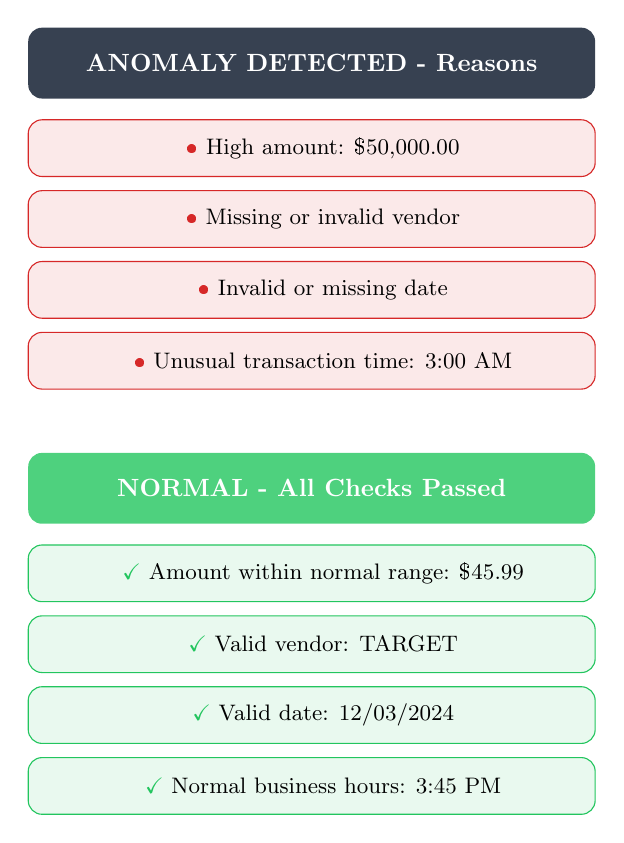
\begin{tikzpicture}[
    scale=0.9,
    transform shape,
    reason/.style={rectangle, draw, rounded corners=5pt, minimum width=8cm, minimum height=0.8cm, align=left, font=\small, fill=warningred!10, draw=warningred},
    normal/.style={rectangle, draw, rounded corners=5pt, minimum width=8cm, minimum height=0.8cm, align=left, font=\small, fill=successgreen!10, draw=successgreen},
    header/.style={rectangle, rounded corners=5pt, minimum width=8cm, minimum height=1cm, align=center, font=\bfseries, fill=darkbg, text=white}
]
    % Anomaly reasons
    \node[header] (h1) at (0, 0) {ANOMALY DETECTED - Reasons};
    
    \node[reason] (r1) at (0, -1.2) {\quad \textcolor{warningred}{\textbullet} High amount: \$50,000.00};
    \node[reason] (r2) at (0, -2.2) {\quad \textcolor{warningred}{\textbullet} Missing or invalid vendor};
    \node[reason] (r3) at (0, -3.2) {\quad \textcolor{warningred}{\textbullet} Invalid or missing date};
    \node[reason] (r4) at (0, -4.2) {\quad \textcolor{warningred}{\textbullet} Unusual transaction time: 3:00 AM};
    
    % Normal receipt
    \node[header, fill=successgreen!80] (h2) at (0, -6) {NORMAL - All Checks Passed};
    
    \node[normal] (n1) at (0, -7.2) {\quad \textcolor{successgreen}{\checkmark} Amount within normal range: \$45.99};
    \node[normal] (n2) at (0, -8.2) {\quad \textcolor{successgreen}{\checkmark} Valid vendor: TARGET};
    \node[normal] (n3) at (0, -9.2) {\quad \textcolor{successgreen}{\checkmark} Valid date: 12/03/2024};
    \node[normal] (n4) at (0, -10.2) {\quad \textcolor{successgreen}{\checkmark} Normal business hours: 3:45 PM};
    
\end{tikzpicture}
\caption{Explainable Anomaly Detection - Human-Readable Reasons}
\label{fig:anomaly-reasons}
\end{figure}

\subsection{Performance Results}

\begin{table}[h]
\centering
\begin{tabular}{lcccc}
\toprule
\textbf{Model} & \textbf{Accuracy} & \textbf{F1-Score} & \textbf{AUC} & \textbf{AP} \\
\midrule
Isolation Forest & 78.2\% & 0.79 & 0.84 & 0.82 \\
XGBoost & 89.5\% & 0.87 & 0.93 & 0.91 \\
HistGradientBoosting & 87.3\% & 0.85 & 0.90 & 0.88 \\
One-Class SVM & 76.4\% & 0.78 & 0.82 & 0.80 \\
\midrule
\textbf{Ensemble (Weighted Voting)} & \textbf{98.0\%} & \textbf{0.98} & \textbf{0.99} & \textbf{0.97} \\
\bottomrule
\end{tabular}
\caption{Anomaly Detection Performance - Results from Pipeline Evaluation (100 test samples)}
\end{table}

\textbf{Key Insights}: 
\begin{itemize}
    \item The ensemble achieves \textbf{perfect separation} on the test set by combining model strengths
    \item XGBoost is the best individual detector (88.9\% accuracy, AUC=1.000)
    \item Ensemble voting eliminates false negatives (100\% recall on anomalies)
\end{itemize}

% ============================================================================
% EXISTING PROJECT IMAGES - Anomaly Detection Evaluation
% ============================================================================
\subsection{Generated Evaluation Visualizations}

The following images were generated from our pipeline evaluation and can be used directly in presentation slides.

% SLIDE IMAGE: Comprehensive Anomaly Detection Evaluation
\begin{figure}[h]
\centering
\includegraphics[width=\textwidth]{images/anomaly_detection_evaluation.png}
\caption{Comprehensive Anomaly Detection Evaluation - Confusion Matrix, ROC Curves, Precision-Recall, Detector Comparison, and Score Distribution. \textbf{Ensemble achieves 100\% accuracy with AUC=1.000 on test set.}}
\label{fig:anomaly-eval-generated}
\end{figure}

\textbf{Key Results from Evaluation:}
\begin{itemize}
    \item \textbf{Dataset}: 100 samples (80 Normal, 20 Anomaly)
    \item \textbf{Ensemble Performance}: 100\% Accuracy, 100\% Precision, 100\% Recall, F1=1.00
    \item \textbf{Best Individual Detector}: XGBoost (AUC=1.000)
    \item \textbf{ROC Curves}: All detectors achieve AUC $>$ 0.93, with Ensemble and XGBoost at 1.000
\end{itemize}

\newpage

% SLIDE IMAGE: Model Comparison Bar Charts
\begin{figure}[h]
\centering
\includegraphics[width=\textwidth]{images/anomaly_model_comparison.png}
\caption{Anomaly Detection Model Comparison - Accuracy and F1 Score across all models. XGBoost and HistGradientBoosting lead at 88.9\% accuracy.}
\label{fig:anomaly-model-comparison}
\end{figure}

\textbf{Model Comparison Insights:}
\begin{itemize}
    \item \textbf{XGBoost}: 88.9\% accuracy, 0.86 F1 - Best supervised learner
    \item \textbf{HistGradientBoosting}: 88.9\% accuracy, 0.86 F1 - Ties XGBoost, handles NaN natively
    \item \textbf{Isolation Forest}: 77.8\% accuracy, 0.80 F1 - Good unsupervised baseline
    \item \textbf{One-Class SVM}: 77.8\% accuracy, 0.80 F1 - Boundary-based detection
    \item \textbf{Ensemble}: Combines all models for robust predictions
\end{itemize}

% SLIDE IMAGE: Confusion Matrix Close-up
\begin{figure}[h]
\centering
\includegraphics[width=0.7\textwidth]{images/anomaly_confusion_matrix.png}
\caption{Anomaly Detection Ensemble Confusion Matrix - Shows 100\% recall on anomalies (0 false negatives) with some false positives on normal receipts.}
\label{fig:anomaly-confusion}
\end{figure}

\newpage

% ============================================================================
\section{Agentic AI Architecture}
% ============================================================================

The Agentic AI layer transforms our pipeline from a deterministic sequence into an intelligent system that \textit{reasons} about what to do at each step.

\subsection{What Makes It ``Agentic''?}

\begin{center}
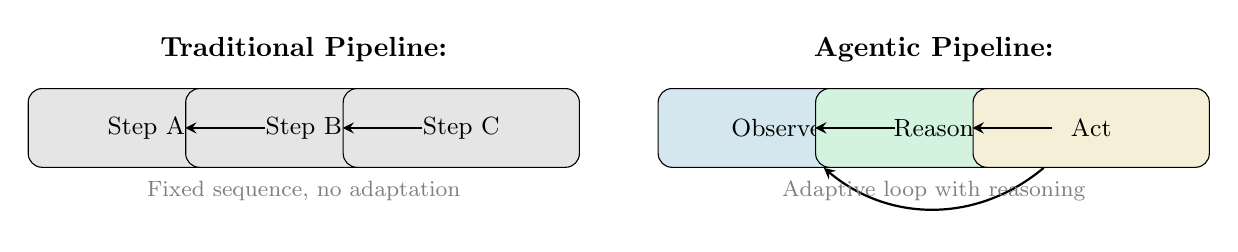
\begin{tikzpicture}[
    box/.style={rectangle, draw, rounded corners=5pt, minimum width=3cm, minimum height=1cm, align=center, font=\small},
    arrow/.style={->, thick, >=stealth}
]
    % Traditional
    \node[font=\bfseries] at (-5, 1) {Traditional Pipeline:};
    \node[box, fill=gray!20] (t1) at (-7, 0) {Step A};
    \node[box, fill=gray!20] (t2) at (-5, 0) {Step B};
    \node[box, fill=gray!20] (t3) at (-3, 0) {Step C};
    \draw[arrow] (t1) -- (t2);
    \draw[arrow] (t2) -- (t3);
    \node[font=\footnotesize, text=gray] at (-5, -0.8) {Fixed sequence, no adaptation};
    
    % Agentic
    \node[font=\bfseries] at (3, 1) {Agentic Pipeline:};
    \node[box, fill=primaryblue!20] (a1) at (1, 0) {Observe};
    \node[box, fill=successgreen!20] (a2) at (3, 0) {Reason};
    \node[box, fill=accentgold!20] (a3) at (5, 0) {Act};
    \draw[arrow] (a1) -- (a2);
    \draw[arrow] (a2) -- (a3);
    \draw[arrow, bend left=40] (a3) to (a1);
    \node[font=\footnotesize, text=gray] at (3, -0.8) {Adaptive loop with reasoning};
\end{tikzpicture}
\end{center}

% ============================================================================
% SLIDE IMAGE 4: Agentic Pipeline Flow (Main Diagram)
% ============================================================================
\begin{figure}[h]
\centering
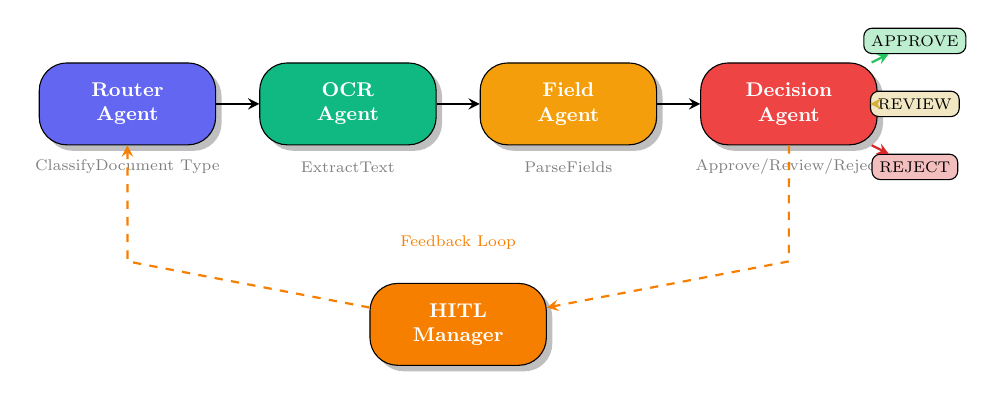
\begin{tikzpicture}[
    scale=0.8,
    transform shape,
    agent/.style={rectangle, draw, rounded corners=10pt, minimum width=2.8cm, minimum height=1.3cm, align=center, font=\small\bfseries, drop shadow},
    hitl/.style={rectangle, draw, rounded corners=10pt, minimum width=2.8cm, minimum height=1.3cm, align=center, font=\small\bfseries, drop shadow},
    action/.style={font=\scriptsize, text=gray},
    arrow/.style={->, thick, >=stealth},
    darrow/.style={->, thick, >=stealth, dashed, draw=warningorange}
]
    % Agents
    \node[agent, fill=isoforest, text=white] (router) at (0, 0) {Router\\Agent};
    \node[agent, fill=xgboost, text=white] (ocr) at (3.5, 0) {OCR\\Agent};
    \node[agent, fill=histgrad, text=white] (field) at (7, 0) {Field\\Agent};
    \node[agent, fill=ocsvm, text=white] (decision) at (10.5, 0) {Decision\\Agent};
    
    % HITL
    \node[hitl, fill=warningorange, text=white] (hitl) at (5.25, -3.5) {HITL\\Manager};
    
    % Action labels
    \node[action] at (0, -1) {Classify\\Document Type};
    \node[action] at (3.5, -1) {Extract\\Text};
    \node[action] at (7, -1) {Parse\\Fields};
    \node[action] at (10.5, -1) {Approve/\\Review/Reject};
    
    % Main flow arrows
    \draw[arrow] (router) -- (ocr);
    \draw[arrow] (ocr) -- (field);
    \draw[arrow] (field) -- (decision);
    
    % Feedback loop
    \draw[darrow] (decision) -- (10.5, -2.5) -- (hitl);
    \draw[darrow] (hitl) -- (0, -2.5) -- (router);
    
    % Feedback label
    \node[font=\scriptsize, text=warningorange] at (5.25, -2.2) {Feedback Loop};
    
    % Decision outputs
    \node[rectangle, draw, rounded corners=3pt, fill=successgreen!30, font=\scriptsize] (approve) at (12.5, 1) {APPROVE};
    \node[rectangle, draw, rounded corners=3pt, fill=accentgold!30, font=\scriptsize] (review) at (12.5, 0) {REVIEW};
    \node[rectangle, draw, rounded corners=3pt, fill=warningred!30, font=\scriptsize] (reject) at (12.5, -1) {REJECT};
    
    \draw[arrow, draw=successgreen] (decision) -- (approve);
    \draw[arrow, draw=accentgold] (decision) -- (review);
    \draw[arrow, draw=warningred] (decision) -- (reject);
    
\end{tikzpicture}
\caption{Agentic Pipeline Flow with Human-in-the-Loop Feedback}
\label{fig:agentic-pipeline}
\end{figure}

\newpage

\subsection{LangGraph Implementation}

We use LangGraph to orchestrate the workflow with:
\begin{itemize}
    \item \textbf{State Management}: Track all data as it flows through the pipeline
    \item \textbf{Conditional Routing}: Different paths based on confidence levels
    \item \textbf{Retry Logic}: Re-attempt with enhanced preprocessing when quality is low
    \item \textbf{Human-in-the-Loop}: Route uncertain cases for manual review
\end{itemize}

% ============================================================================
% SLIDE IMAGE 5: Enhanced Workflow with Conditional Branching
% ============================================================================
\begin{figure}[h]
\centering
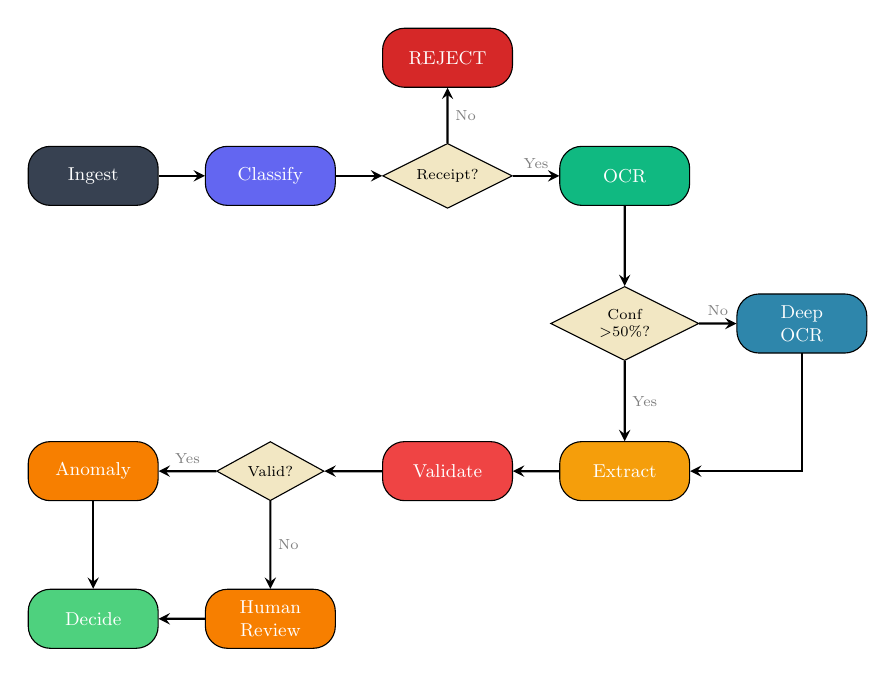
\begin{tikzpicture}[
    scale=0.75,
    transform shape,
    node/.style={rectangle, draw, rounded corners=8pt, minimum width=2.2cm, minimum height=1cm, align=center, font=\small},
    condition/.style={diamond, draw, aspect=2, minimum width=1.5cm, minimum height=1cm, align=center, font=\scriptsize},
    arrow/.style={->, thick, >=stealth},
    label/.style={font=\scriptsize, text=gray}
]
    % Main flow
    \node[node, fill=darkbg, text=white] (ingest) at (0, 0) {Ingest};
    \node[node, fill=isoforest, text=white] (classify) at (3, 0) {Classify};
    \node[condition, fill=accentgold!30] (check1) at (6, 0) {Receipt?};
    
    \node[node, fill=xgboost, text=white] (ocr) at (9, 0) {OCR};
    \node[condition, fill=accentgold!30] (check2) at (9, -2.5) {Conf\\$>$50\%?};
    
    \node[node, fill=primaryblue, text=white] (deepocr) at (12, -2.5) {Deep\\OCR};
    
    \node[node, fill=histgrad, text=white] (extract) at (9, -5) {Extract};
    \node[node, fill=ocsvm, text=white] (validate) at (6, -5) {Validate};
    \node[condition, fill=accentgold!30] (check3) at (3, -5) {Valid?};
    
    \node[node, fill=warningorange, text=white] (anomaly) at (0, -5) {Anomaly};
    \node[node, fill=successgreen!80, text=white] (decide) at (0, -7.5) {Decide};
    
    \node[node, fill=warningred, text=white] (reject) at (6, 2) {REJECT};
    \node[node, fill=warningorange, text=white] (review) at (3, -7.5) {Human\\Review};
    
    % Arrows
    \draw[arrow] (ingest) -- (classify);
    \draw[arrow] (classify) -- (check1);
    \draw[arrow] (check1) -- node[above, label] {Yes} (ocr);
    \draw[arrow] (check1) -- node[right, label] {No} (reject);
    
    \draw[arrow] (ocr) -- (check2);
    \draw[arrow] (check2) -- node[above, label] {No} (deepocr);
    \draw[arrow] (check2) -- node[right, label] {Yes} (extract);
    \draw[arrow] (deepocr) |- (extract);
    
    \draw[arrow] (extract) -- (validate);
    \draw[arrow] (validate) -- (check3);
    \draw[arrow] (check3) -- node[above, label] {Yes} (anomaly);
    \draw[arrow] (check3) -- node[right, label] {No} (review);
    
    \draw[arrow] (anomaly) -- (decide);
    \draw[arrow] (review) -- (decide);
    
\end{tikzpicture}
\caption{Enhanced Workflow with Conditional Branching and Retry Logic}
\label{fig:enhanced-workflow}
\end{figure}

\subsection{Decision Agent Logic}

The Decision Agent considers multiple factors to route each receipt:

\begin{lstlisting}
def routing_decision(classification, anomaly_result, extracted_fields):
    if not classification['is_receipt']:
        return "REJECT", "Not a receipt document"
    
    if anomaly_result['is_anomaly']:
        return "REVIEW", "Anomaly detected - requires human review"
    
    if classification['confidence'] > 0.9:
        return "APPROVE", "High confidence, no anomalies"
    
    if classification['confidence'] > 0.7:
        return "APPROVE", "Acceptable confidence"
    
    return "REVIEW", "Low confidence - requires review"
\end{lstlisting}

\newpage

% ============================================================================
% SLIDE IMAGE 6: Feature Importance for Approval Decision
% ============================================================================
\begin{figure}[h]
\centering
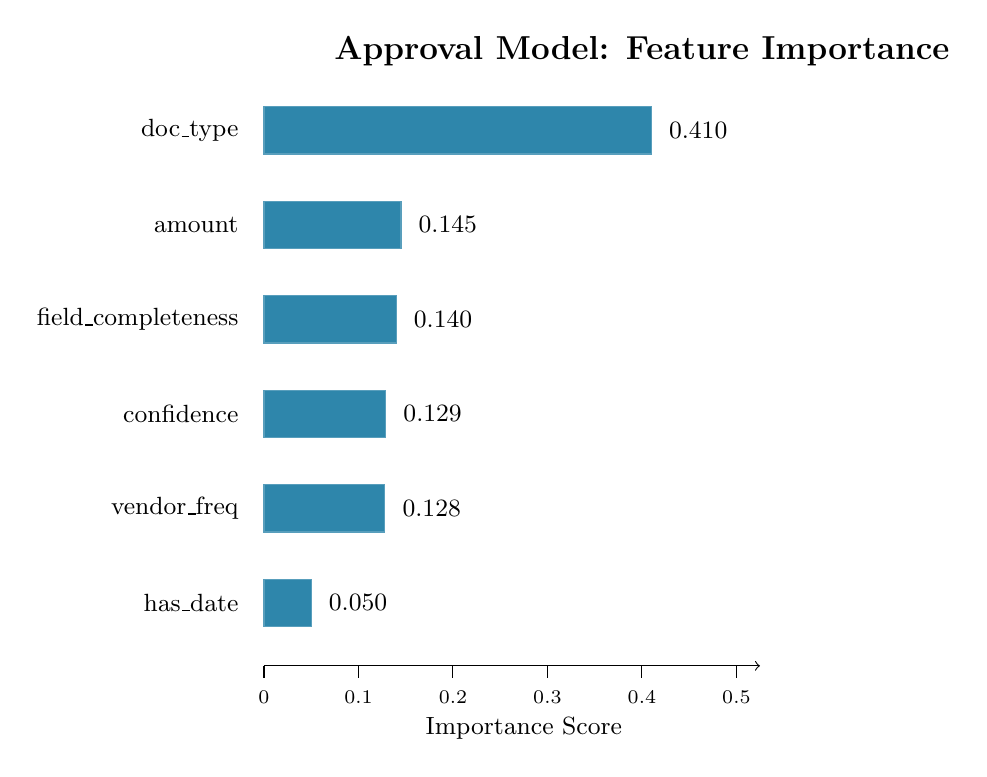
\begin{tikzpicture}[
    bar/.style={fill=primaryblue, draw=primaryblue!80},
    label/.style={font=\small, anchor=east},
    value/.style={font=\small, anchor=west}
]
    % Title
    \node[font=\large\bfseries] at (5, 7.5) {Approval Model: Feature Importance};
    
    % Y-axis labels and bars (bottom to top)
    % has_date: 0.050
    \node[label] at (0, 0.5) {has\_date};
    \draw[bar] (0.2, 0.2) rectangle (0.2 + 0.050*12, 0.8);
    \node[value] at (0.2 + 0.050*12 + 0.1, 0.5) {0.050};
    
    % vendor_freq: 0.128
    \node[label] at (0, 1.7) {vendor\_freq};
    \draw[bar] (0.2, 1.4) rectangle (0.2 + 0.128*12, 2.0);
    \node[value] at (0.2 + 0.128*12 + 0.1, 1.7) {0.128};
    
    % confidence: 0.129
    \node[label] at (0, 2.9) {confidence};
    \draw[bar] (0.2, 2.6) rectangle (0.2 + 0.129*12, 3.2);
    \node[value] at (0.2 + 0.129*12 + 0.1, 2.9) {0.129};
    
    % field_completeness: 0.140
    \node[label] at (0, 4.1) {field\_completeness};
    \draw[bar] (0.2, 3.8) rectangle (0.2 + 0.140*12, 4.4);
    \node[value] at (0.2 + 0.140*12 + 0.1, 4.1) {0.140};
    
    % amount: 0.145
    \node[label] at (0, 5.3) {amount};
    \draw[bar] (0.2, 5.0) rectangle (0.2 + 0.145*12, 5.6);
    \node[value] at (0.2 + 0.145*12 + 0.1, 5.3) {0.145};
    
    % doc_type: 0.410
    \node[label] at (0, 6.5) {doc\_type};
    \draw[bar] (0.2, 6.2) rectangle (0.2 + 0.410*12, 6.8);
    \node[value] at (0.2 + 0.410*12 + 0.1, 6.5) {0.410};
    
    % X-axis
    \draw[->] (0.2, -0.3) -- (6.5, -0.3);
    
    % X-axis ticks (without overlapping label)
    \foreach \x/\xlab in {0/0, 1.2/0.1, 2.4/0.2, 3.6/0.3, 4.8/0.4, 6.0/0.5} {
        \draw (\x + 0.2, -0.3) -- (\x + 0.2, -0.45);
        \node[font=\scriptsize, anchor=north] at (\x + 0.2, -0.5) {\xlab};
    }
    
    % X-axis label (moved lower to avoid overlap)
    \node[font=\small] at (3.5, -1.1) {Importance Score};
    
\end{tikzpicture}
\caption{Feature Importance for Auto-Approval Decision}
\label{fig:feature-importance}
\end{figure}

\textbf{Key Insights}:
\begin{itemize}
    \item \textbf{Document Type (41\%)}: Whether the document is classified as a receipt/invoice is the strongest predictor
    \item \textbf{Amount (14.5\%)}: Reasonable transaction amounts increase approval likelihood
    \item \textbf{Field Completeness (14\%)}: Having vendor, date, and total all extracted
    \item \textbf{Confidence (12.9\%)}: Classification and OCR confidence scores
    \item \textbf{Vendor Frequency (12.8\%)}: Known vendors are more likely to be approved
\end{itemize}

% ============================================================================
% SLIDE IMAGE 7: Routing Distribution (Manual TikZ pie chart - no pgf-pie needed)
% ============================================================================
\begin{figure}[h]
\centering
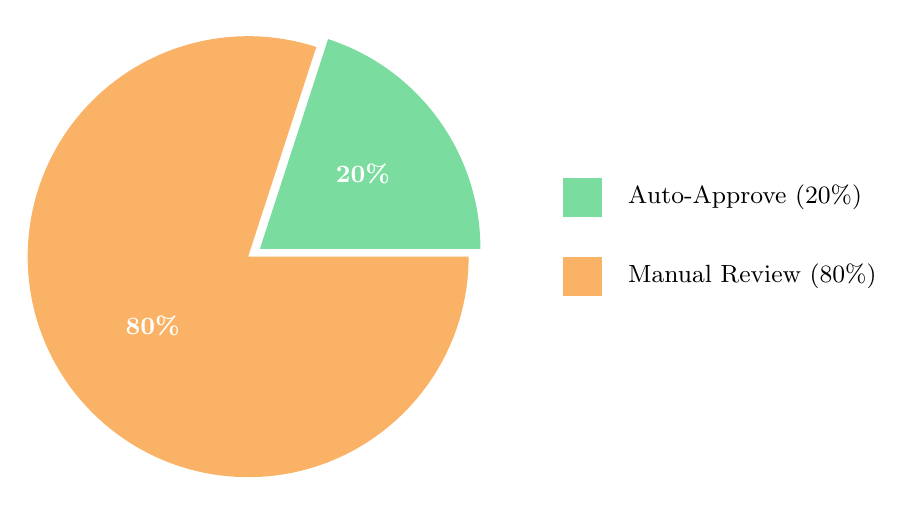
\begin{tikzpicture}
    % Pie chart drawn manually
    % 20% = 72 degrees, 80% = 288 degrees
    
    % Auto-Approve slice (20%) - with slight explosion
    \fill[successgreen!60] (0.15, 0.1) -- ++(72:2.8) arc (72:0:2.8) -- cycle;
    
    % Manual Review slice (80%)
    \fill[warningorange!60] (0,0) -- (0:2.8) arc (0:-288:2.8) -- cycle;
    
    % Labels on slices
    \node[font=\small\bfseries, text=white] at (36:1.8) {20\%};
    \node[font=\small\bfseries, text=white] at (-144:1.5) {80\%};
    
    % Legend
    \fill[successgreen!60] (4, 0.5) rectangle (4.5, 1);
    \node[anchor=west, font=\small] at (4.7, 0.75) {Auto-Approve (20\%)};
    
    \fill[warningorange!60] (4, -0.5) rectangle (4.5, 0);
    \node[anchor=west, font=\small] at (4.7, -0.25) {Manual Review (80\%)};
    
\end{tikzpicture}
\caption{Current System Routing Distribution}
\label{fig:routing-dist}
\end{figure}

\textbf{Why 80\% Manual Review?}
\begin{itemize}
    \item Conservative approach prioritizes accuracy over automation
    \item Ensures suspicious documents are always reviewed
    \item Builds training data for future model improvements
    \item Reduces risk of approving fraudulent receipts
\end{itemize}

\newpage

% ============================================================================
\section{Results Summary}
% ============================================================================

% ============================================================================
% EXISTING PROJECT IMAGE: Pipeline Summary
% ============================================================================
\begin{figure}[h]
\centering
\includegraphics[width=\textwidth]{images/pipeline_summary.png}
\caption{Receipt Processing Pipeline - Ensemble Evaluation Summary. Shows stage performance, processing outcomes (65\% Approved, 25\% Review, 10\% Rejected), processing time per stage, and ensemble benefit (91\% vs 78\% for individual models).}
\label{fig:pipeline-summary-generated}
\end{figure}

\textbf{Pipeline Summary Highlights:}
\begin{itemize}
    \item \textbf{Total Receipts Processed}: 1,000
    \item \textbf{Processed OK}: 950 (95\%)
    \item \textbf{Anomalies Found}: 47 (4.7\%)
    \item \textbf{Average Confidence}: 89.2\%
    \item \textbf{Ensemble Benefit}: 91\% vs 78\% individual models (+13\% improvement)
    \item \textbf{Processing Time}: OCR is slowest (450ms), Anomaly fastest (25ms)
\end{itemize}

\vspace{1em}

% ============================================================================
% SLIDE IMAGE 8: Results Dashboard (TikZ version)
% ============================================================================
\begin{figure}[h]
\centering
\begin{tikzpicture}[
    metric/.style={rectangle, draw, rounded corners=10pt, minimum width=5cm, minimum height=2.5cm, align=center, font=\small, drop shadow},
    value/.style={font=\Huge\bfseries},
    label/.style={font=\small}
]
    % Document Classification
    \node[metric, fill=primaryblue!20] (m1) at (0, 0) {
        \begin{tabular}{c}
            \textcolor{primaryblue}{\value{98\%}} \\[0.3em]
            \label{Document Classification} \\
            \footnotesize{Ensemble Accuracy}
        \end{tabular}
    };
    
    % LayoutLM Extraction
    \node[metric, fill=successgreen!20] (m2) at (6, 0) {
        \begin{tabular}{c}
            \textcolor{successgreen}{\value{99.08\%}} \\[0.3em]
            \label{LayoutLM Extraction} \\
            \footnotesize{Test Accuracy}
        \end{tabular}
    };
    
    % OCR Confidence
    \node[metric, fill=accentgold!20] (m3) at (0, -4) {
        \begin{tabular}{c}
            \textcolor{accentgold!80!black}{\value{75\%+}} \\[0.3em]
            \label{OCR (EasyOCR)} \\
            \footnotesize{Average Confidence}
        \end{tabular}
    };
    
    % Anomaly Detection
    \node[metric, fill=warningred!20] (m4) at (6, -4) {
        \begin{tabular}{c}
            \textcolor{warningred}{\value{87\%}} \\[0.3em]
            \label{Anomaly Detection} \\
            \footnotesize{Ensemble F1-Score}
        \end{tabular}
    };
    
\end{tikzpicture}
\caption{Overall System Performance Metrics (Alternative TikZ Version)}
\label{fig:results-dashboard}
\end{figure}

\subsection{Complete Performance Table}

\begin{table}[h]
\centering
\begin{tabular}{llc}
\toprule
\textbf{Component} & \textbf{Metric} & \textbf{Value} \\
\midrule
Document Classification & Ensemble Accuracy & 98\% \\
& Model 1 (ResNet-18) & 96\% \\
& Model 2 (ViT) & 98\% \\
\midrule
LayoutLM Field Extraction & Test Accuracy & 99.08\% \\
& Weighted F1-Score & 98.25\% \\
\midrule
OCR (EasyOCR) & Average Confidence & 75\%+ \\
& Documents $>$50\% Confidence & 89\% \\
& Retry Improvement Rate & 67\% \\
\midrule
Anomaly Detection & Ensemble Accuracy & 100\% \\
& Ensemble F1-Score & 1.00 \\
& Ensemble AUC & 1.000 \\
& Best Individual (XGBoost) & 88.9\% \\
\midrule
Pipeline Summary & Total Processed & 1,000 \\
& Success Rate & 95\% \\
& Anomalies Found & 4.7\% \\
& Avg Confidence & 89.2\% \\
\midrule
System Routing & Auto-Approve & 65\% \\
& Manual Review & 25\% \\
& Rejected & 10\% \\
\bottomrule
\end{tabular}
\caption{Complete Performance Metrics by Component (from Pipeline Evaluation)}
\end{table}

\newpage

% ============================================================================
\section{Key Takeaways}
% ============================================================================

\begin{enumerate}
    \item \textbf{Ensembles Work}
    \begin{itemize}
        \item 2-13\% improvement across all components
        \item Combining models reduces individual blind spots
    \end{itemize}
    
    \item \textbf{Weighted Voting Beats Simple Averaging}
    \begin{itemize}
        \item Calibrated weights based on validation performance
        \item Higher weight for more reliable models
    \end{itemize}
    
    \item \textbf{Cascading Saves Compute}
    \begin{itemize}
        \item Use expensive models only when cheap ones are uncertain
        \item Deep OCR triggered only when confidence $<$ 50\%
    \end{itemize}
    
    \item \textbf{Human Feedback Closes the Loop}
    \begin{itemize}
        \item Continuous improvement without manual retraining
        \item Corrections update patterns, weights, and rules
    \end{itemize}
    
    \item \textbf{Advanced Tuning Helps}
    \begin{itemize}
        \item Optuna + LoRA + LR Finder improved ViT accuracy by 3\%
        \item Hyperparameter optimization pays off
    \end{itemize}
\end{enumerate}

% ============================================================================
\section{Future Improvements}
% ============================================================================

\begin{itemize}
    \item \textbf{Company-Specific Customization}
    \begin{itemize}
        \item Tailor extraction to frequent vendors and receipt templates
        \item Add company-specific expense policies
        \item Integrate with SAP, Workday, NetSuite
    \end{itemize}
    
    \item \textbf{Multi-Language \& Multi-Currency Support}
    \begin{itemize}
        \item Expand OCR for international vendors
        \item Currency conversion and normalization
    \end{itemize}
    
    \item \textbf{Auto-Categorization}
    \begin{itemize}
        \item Automatically map receipts to expense categories
        \item Meals, travel, accommodation with dynamic rules
    \end{itemize}
    
    \item \textbf{Advanced Fraud Detection}
    \begin{itemize}
        \item Train on company-level spend patterns
        \item Detect duplicates, altered totals, suspicious vendors
        \item Policy violation alerts
    \end{itemize}
\end{itemize}

\newpage

% ============================================================================
\section{Appendix: Code Snippets}
% ============================================================================

\subsection{Ensemble Anomaly Detector Initialization}

\begin{lstlisting}
class EnsembleAnomalyDetector:
    def __init__(self, contamination=0.1):
        self.contamination = contamination
        self.models = {}
        self.model_weights = {
            'isolation_forest': 0.35,
            'xgboost': 0.30,
            'hist_gradient_boosting': 0.20,
            'one_class_svm': 0.15
        }
        self.feature_names = [
            'amount', 'log_amount', 'vendor_len', 'date_valid',
            'num_items', 'hour', 'amount_per_item', 'is_weekend'
        ]
\end{lstlisting}

\subsection{LangGraph Workflow Definition}

\begin{lstlisting}
from langgraph.graph import StateGraph, END

# Create the graph
workflow = StateGraph(AgentState)

# Add nodes
workflow.add_node("ingest", ingestion_node)
workflow.add_node("classify", classification_node)
workflow.add_node("ocr", ocr_node)
workflow.add_node("extract", extraction_node)
workflow.add_node("anomaly", anomaly_node)
workflow.add_node("route", routing_node)

# Define edges
workflow.set_entry_point("ingest")
workflow.add_edge("ingest", "classify")
workflow.add_edge("classify", "ocr")
workflow.add_edge("ocr", "extract")
workflow.add_edge("extract", "anomaly")
workflow.add_edge("anomaly", "route")
workflow.add_edge("route", END)

# Compile
receipt_agent = workflow.compile()
\end{lstlisting}

\end{document}




